\documentclass[border=0pt]{standalone}
\usepackage{fontspec}
\setmainfont{Carlito}
\usepackage{unicode-math}
\setmathfont{Latin Modern Math}
\usepackage{xcolor}
\usepackage{booktabs}
\usepackage{tikz}
\usepackage{graphicx}

\definecolor{canvabg}{RGB}{246,244,241}
\definecolor{textDark}{RGB}{40,40,40}
\definecolor{textMute}{RGB}{125,120,113}
\definecolor{accent}{RGB}{18,125,108}
\definecolor{trough}{RGB}{160,55,50}
\definecolor{bridge}{RGB}{30,90,140}

\pagecolor{canvabg}

\providecommand{\Cref}[1]{}
\providecommand{\cref}[1]{}
\providecommand{\ab}[1]{#1}

\renewcommand{\arraystretch}{1.45}

\begin{document}
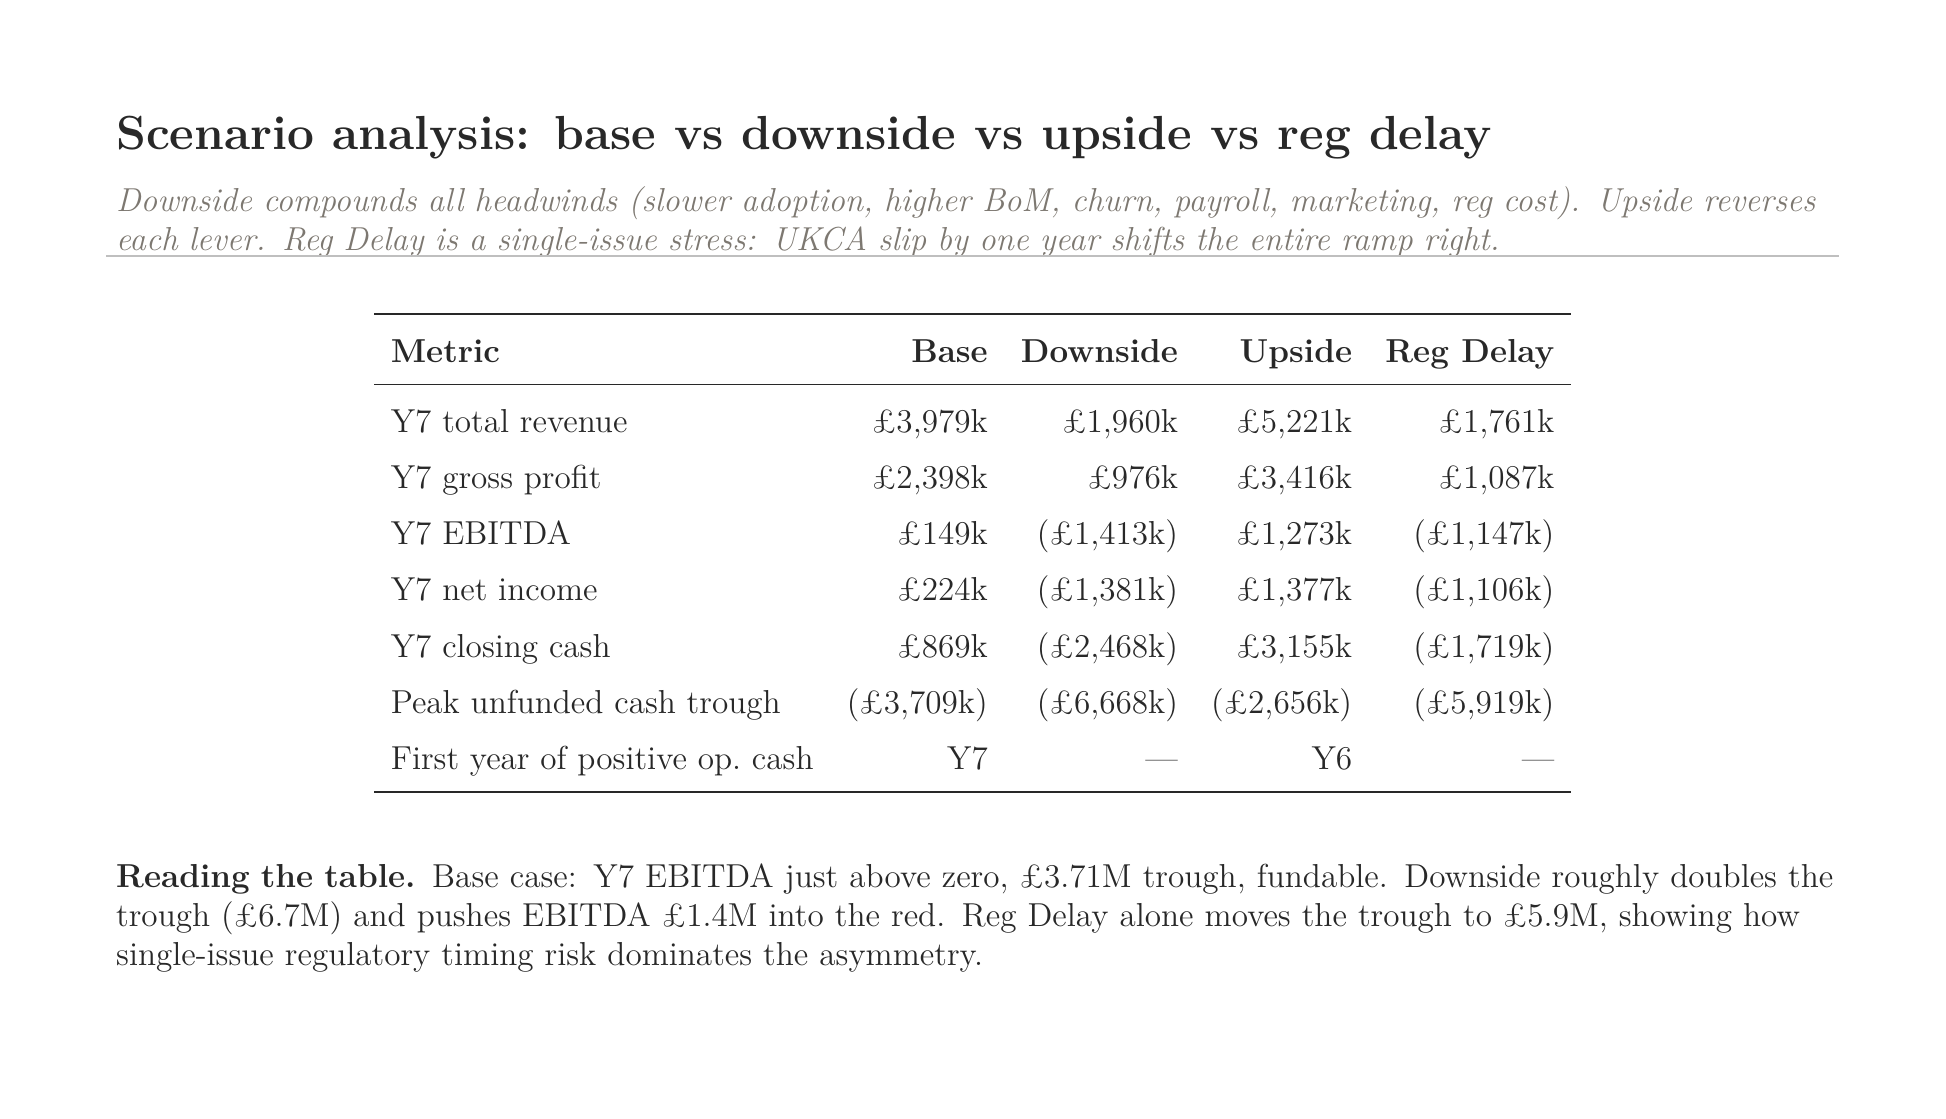
\begin{tikzpicture}[every node/.style={text=textDark}]
\useasboundingbox (0,0) rectangle (24, 13.5);

\node[anchor=north west, font=\bfseries\LARGE] at (1.0, 12.5)
    {Scenario analysis: base vs downside vs upside vs reg delay};
\node[anchor=north west, font=\itshape\large, text=textMute, text width=22cm]
    at (1.0, 11.6)
    {Downside compounds all headwinds (slower adoption, higher BoM, churn,
     payroll, marketing, reg cost). Upside reverses each lever. Reg Delay is
     a single-issue stress: UKCA slip by one year shifts the entire ramp right.};

\draw[gray!50, line width=0.5pt] (1.0, 10.6) -- (23.0, 10.6);

\node[anchor=north, font=\large] at (12.0, 10.0) {%
\begin{tabular}{lrrrr}
    \toprule
    \textbf{Metric} & \textbf{Base} & \textbf{Downside} & \textbf{Upside} & \textbf{Reg Delay} \\
    \midrule
    Y7 total revenue                  & \pounds 3{,}979k    & \pounds 1{,}960k    & \pounds 5{,}221k    & \pounds 1{,}761k \\
    Y7 gross profit                   & \pounds 2{,}398k    & \pounds 976k          & \pounds 3{,}416k    & \pounds 1{,}087k \\
    Y7 EBITDA                         & \pounds 149k          & (\pounds 1{,}413k)  & \pounds 1{,}273k    & (\pounds 1{,}147k) \\
    Y7 net income                     & \pounds 224k          & (\pounds 1{,}381k)  & \pounds 1{,}377k    & (\pounds 1{,}106k) \\
    Y7 closing cash                   & \pounds 869k          & (\pounds 2{,}468k)  & \pounds 3{,}155k    & (\pounds 1{,}719k) \\
    Peak unfunded cash trough         & (\pounds 3{,}709k)  & (\pounds 6{,}668k)  & (\pounds 2{,}656k)  & (\pounds 5{,}919k) \\
    First year of positive op.\ cash  & Y7                    & ---                   & Y6                    & --- \\
    \bottomrule
\end{tabular}
};

\node[anchor=north west, text width=22cm, font=\large] at (1.0, 3.0)
    {\textbf{Reading the table.} Base case: Y7 EBITDA just above zero,
     \pounds 3.71M trough, fundable. Downside roughly doubles the trough
     (\pounds 6.7M) and pushes EBITDA \pounds 1.4M into the red. Reg Delay
     alone moves the trough to \pounds 5.9M, showing how single-issue
     regulatory timing risk dominates the asymmetry.};

\end{tikzpicture}
\end{document}
